\documentclass[FM,BP]{tulthesis}
\usepackage{polyglossia}
\setdefaultlanguage{czech}
\usepackage{xevlna}
\usepackage{graphicx}
\usepackage{amsmath}
\usepackage{siunitx}

\usepackage{makeidx}
\makeindex

% fonty
\usepackage{fontspec}
\usepackage{xunicode}
\usepackage{xltxtra}
%\setmainfont[Mapping=textext,BoldFont={* Bold},Numbers=OldStyle]{Baskerville 10 Pro}
%\setsansfont[Mapping=textext,BoldFont={* Bold},Numbers=OldStyle]{Myriad Pro}
%\setmonofont[Scale=MatchLowercase]{Vida Mono 32 Pro}

% příkazy specifické pro tento dokument
\newcommand{\argument}[1]{{\ttfamily\color{\tulcolor}#1}}
\newcommand{\argumentindex}[1]{\argument{#1}\index{#1}}
\newcommand{\prostredi}[1]{\argumentindex{#1}}
\newcommand{\prikazneindex}[1]{\argument{\textbackslash #1}}
\newcommand{\prikaz}[1]{\prikazneindex{#1}\index{#1@\textbackslash #1}}
\newenvironment{myquote}{\begin{list}{}{\setlength\leftmargin\parindent}\item[]}{\end{list}}
\newenvironment{listing}{\begin{myquote}\color{\tulcolor}}{\end{myquote}}
\sloppy

% deklarace pro titulní stránku

\TULtitle{VPython/GlowScript Trinket ve výuce fyziky}{}
\TULprogramme{N2612}{Elektrotechnika~a~informatika}{Electrical engineering and informatics}
\TULbranch{1802T007}{Informační technologie}{Information technology}
\TULauthor{Aliaksei Kalosha}
\TULsupervisor{Martin Huněk}
\TULyear{2020}

% Vložil Koprnický, použití bibLateXu
\usepackage[ 
backend=biber
%,style=iso-authoryear
,style=iso-numeric
%,style=numeric
%,sortlocale=cs_CZ
,autolang=other
,bibencoding=UTF8
%,urldate=edtf
]{biblatex}
\addbibresource{citace.bib} % vložení seznamu literárních zdrojů~v~bib formátu

\usepackage{csquotes} %užití biblatexu hlasí warnings, důvodem může být použití českých uvozovek~v~citacích!
\urlstyle{same} %sazba url odkazů stejným fontem jako ostatní text, řešení problémů~v~zalamování hypertextových odkazů~v~citacích

\begin{document}


\ThesisStart{male}
%\ThesisStart{zadaniaprohlaseni.pdf}

\begin{abstractCZ}~V~současné době, se klade velký důraz na vizualizaci všech abstraktních pojmů, jak ve vzdělávání, tak~i~v běžném životě. Tento fakt je učitelům fyziky dávno znám. Někteří učitelé svým žákům~a~studentům svoje vlastní vizualizace nabízí/vytváří. Podobnou službu nabízí vizualizační programy od specializovaných vzdělávacích firem. Cílem tohoto příspěvku je představit jedno takové prostředí, ve kterém mohou, jak učitelé, tak~i~žáci, zdarma~a~na různých platformách vytvářet fyzikální vizualizace.
\end{abstractCZ}

\begin{keywordsCZ}
vizualizaci, abstraktní pojmy
\end{keywordsCZ}

\vspace{2cm}


\clearpage

\begin{acknowledgement}
Rád bych poděkoval všem, kteří přispěli ke vzniku tohoto dílka.
\end{acknowledgement}

\tableofcontents
\listoffigures
\listoftables

\chapter{Úvod}
Vizuální stránka hraje ve společnosti~v~posledních několika letech velmi výraznou roli. To se podepisuje také na tom, že je kladen mnohem větší důraz na to, jak prezentovat informace, než jaké informace se prezentují. To je ale~v~přímém rozporu~s~tím, jak obrazovou reprezentaci vnímají přírodovědci. Ti kladou důraz na maximální přesnost~a~adekvátní množstvísdělovaných informací. Didaktici mimo vědecké přesnosti požadují názornost přiměřenou mentální úrovni žáků.

Vizualizace ve vzdělávání je důležitá~i~z toho důvodu, že člověk přijímácca 80\% informací ze svého okolí zrakem \cite{c:1}. Pokud chceme, aby si tatodata pamatoval, pak je účinnost takového procesu 40\% \cite{c:1}. Dalšími cílivizualizace je získat pozornost žáka, zaujmout žáka, sdělit nové informacežákovi, názornost probírané látky. Vizualizační prostředky lze využít vevšech fázích vyučovací hodiny. Od motivační fáze, až po fázi diagnostickou.Shrnemeli si předchozí, pak lze říci, že žáci si za pomoci vizuálií lépezasazují informace do správného kontextu \cite{c:2}.
~K~vlastní vizualizaci,~v~našem případě budeme hovořit~o~modelech fyzikální podstaty, lze využívat různá vývojová prostředí, ve kterých mohoupracovat jak vědci, učitelé, tak jejich žáci~a~studenti. Některými~z~nichjsou například Famulus, IP Coach, Algodoo (dříve Phun), PHP, HTML5,Mathematica, Easy Java Simulations, Modellus, VPython~a~nebo jehozcela otevřená varianta GlowScript Trinket. Poslednímu zmíněnému prostředí, GlowScript Trinket, se budeme~v~tomto příspěvku věnovat blíže \cite{c:3}.

\chapter{VPython/GlowScript Trinket}
Prostředí VPython, které~v~roce 2000 vytvořil D. Scherer, umožňujevytváření 3D zobrazení~a~animací,~a~to~i~těm, kteří mají omezené zkušenosti~s~programováním. Prostředí je založeno na klasickém Pythonu, dokážís ním proto pracovat zkušení programátoři~i~vědci. Pro pohodlnější práci atvorbu animací vytvořili~v~roce 2011 D. Scherer~a~B. Sherwood GlowScript,který vychází~z~programové základny Pythonu, používá grafické knihovnyVPythonu, ale na rozdíl od nich ho lze provozovat ve webovém prohlížečia to jak tvorbu zdrojového kódu, tak~i~jeho výstup. Prostředí Trinket,které pracuje se stejnou syntaxí jako GlowScript, pak~v~roce 2003 vytvořilE. Hauser. Výhodné je, že je možné užívat totéž prostředí jak ve škole, taki doma,~a~to bezplatně na straně žáka/studenta \cite{c:4,c:5,c:6}.

VPython/GlowScript má výhodu~v~tom, že~v~něm lze modelovat například pohyb těles, pohyb elektronů obvodem~a~mnoho dalšího. Současně lzevykreslovat průběh veličin, které jsou~v~animaci měněny~a~pomocí matematických vztahů zapisovány. Tuto vlastnost tak lze využít jak~v~kvalitativní, tak~i~v kvantitativním přiblížení nového učiva napříč všemi úrovněmiškolního vzdělávání. Například na prvním stupni základní školy můžemežákům demonstrovat pohyb planet Sluneční soustavy kvalitativně, zatímcona druhém stupni základní školy již můžeme nechat vykreslovat průběhrychlosti planet~v~jednotlivých fázích oběhu kolem Slunce \ref{obr1}. Dále lzeanimaci přiblížit nebo naopak oddálit případně jinak~s~objekty manipulovat. Žáci mohou modelovanou situaci digitálně prozkoumat~z~více úhlůpohledu. Lze tak tedy celý systém sledovat komplexně nebo jenom některéčást izolovaně, což napomáhá lepšímu porozumění zkoumaných jevů.

\begin{figure}[ht]
\centering
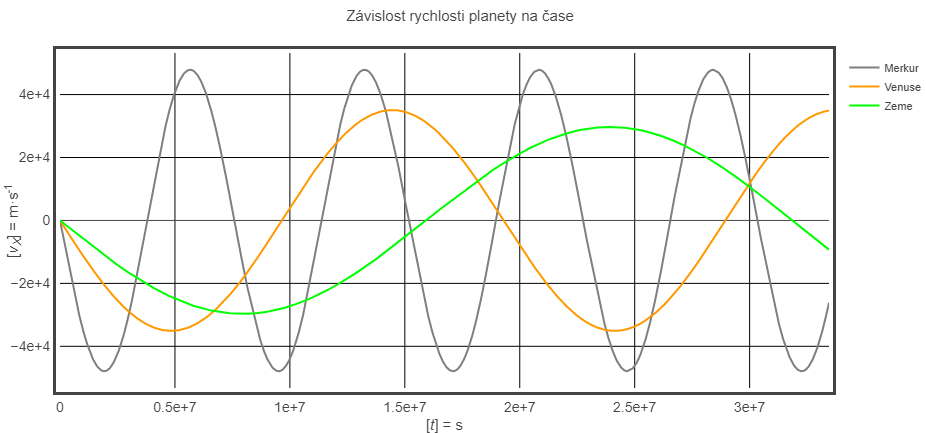
\includegraphics[width=\textwidth]{img1.png}
\caption{Graf závislosti $x$-ové složky rychlosti planet Merkur, Venuše, Země načase}
\label{obr1}
\end{figure}
Protože se jedná~o~prostředí, které je primárně vytvořeno pro demonstraci fyzikálních jevů, vytvořili autoři programu sami knihovnu, ve kteréjsou předvytvořené některé objekty, se kterými se ve fyzice setkáváme. Aťuž se jedná~o~klasická tělesa (koule, krychle, válce), ale~i~šipky, pružinu,jehlan, kruh~a~další.Z tohoto pohledu tak pro tvůrce modelu/vizualizace odpadá nutnostpřemýšlet~a~vytvářet vlastní modely pomocí zápisu kódu jednotlivýchprvků, ale může se více soustředit na fyzikální podstatu problému.Pokud se zaměříme na tvorbu modelů~z~pohledu učitele, tak na ni budejistě nahlížet~z~několika úhlů~a~to~z~didaktického, fyzikálního, technickéhoa programátorského.
\begin{figure}[ht]
\centering
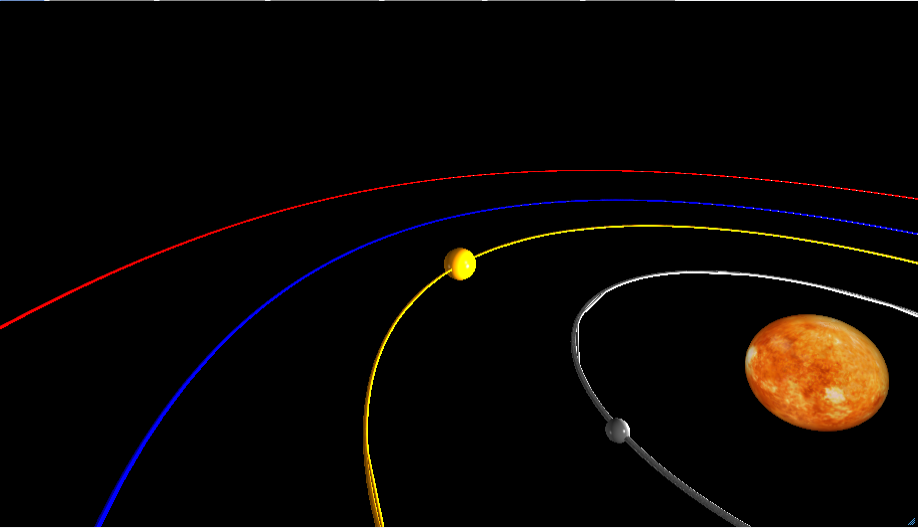
\includegraphics[width=\textwidth]{img2.png}
\caption{Pohled na model Sluneční soustavy – kamenné planety, detail na Merkura Venuši. (Vidíme, že přivrácené strany planet ke Slunci jsou jím osvícené.)}
\label{obr2}
\end{figure}
\begin{figure}[ht]
\centering
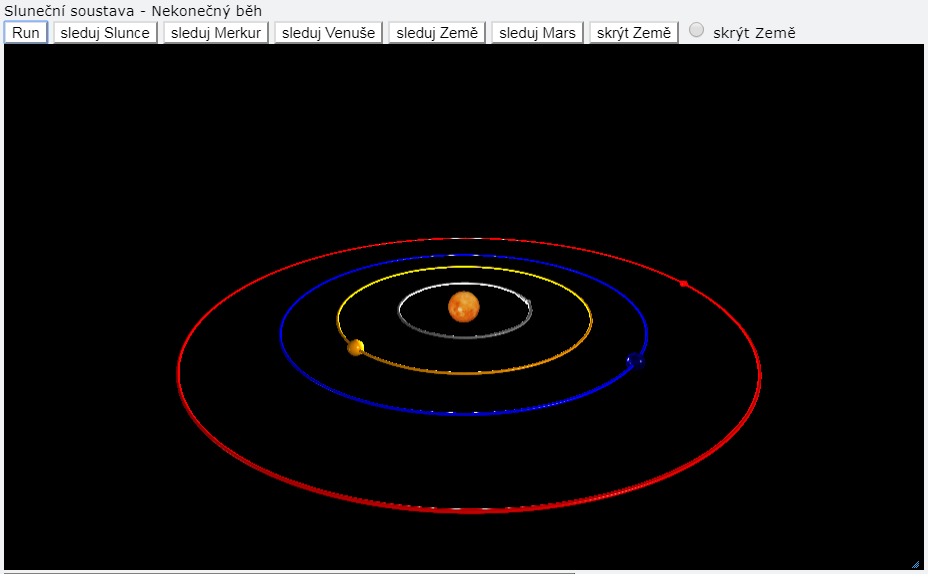
\includegraphics[width=\textwidth]{img3.png}
\caption{Pohled na model Sluneční soustavy – kamenné planety}
\label{obr3}
\end{figure}
\section{Didaktické hledisko}
Pokud se nyní nebudeme soustředit na tvorbu, ale již na prezentacihotových modelů, pak je vhodné poznamenat, že~z~didaktického hlediskase jedná~o~vhodný nástroj. Jak je již uvedeno výše,~s~modely lze různěmanipulovat (pohybovat, natáčet, přibližovat/oddalovat), což umožňujezkoumání jednotlivých detailů (viz \ref{obr2}). Nebo naopak se od nich oprostíme~a~budeme systém sledovat jako celek, tedy "z dálky" (viz \ref{obr3}).

Další výhodou je možnost práce se světlem, což opět napomáhá realistickému efektu zkoumaného jevu (například Sluneční soustava). Žáci tak mohou studovat pohyb planet kolem Slunce,~a~jak tento jev souvisí sestřídáním dne~a~noci nebo~z~pohybu Měsíce kolem Země si vysvětlit zatmění Slunce~a~Měsíce. Pohyby těchto vesmírných těles můžeme modelovatpomocí matematického zápisu fyzikální podstaty jevu.

Na tomto místě je vhodné poznamenat, že nejčastěji se používají jednoduché matematické postupy ve chvílích, kdy je analytické řešení problémužákovi cizí nebo je pro něj právě matematicky náročné. Tento postup jeodborné veřejnosti znám jako dynamické modelování. Dynamické modelování využívá toho, že autor umí fyzikálně~a~matematicky popsat daný jev adokáže diferenciální rovnice komplexně popisující děj vyřešit~a~přepsat natakové vztahy, kdy jsou veličiny získávány na základě funkce času.~K~tomupotřebujeme znát také počáteční podmínky popisující systém \cite{c:3,c:7,c:8,c:9}.
\section{Fyzikální hledisko}
Vyjdeme ze dvou základních faktů, se kterými přicházejí žáci~z~mateřských škol (dále MŠ) do škol základních (dále ZŠ)~a~to, že:
\begin{enumerate}
    \item Země má jednu přirozenou družici, Měsíc,
    \item dvojice Země–Měsíc obíhá kolem Slunce.
\end{enumerate}

Pro první přiblížení pro žáky~v~MŠ, ale~i~na 1. stupni ZŠ, bude stačit,když sdělíme, že vzdálenosti~a~hmotnosti všech tří vesmírných těles nabývají takových hodnot, že setrvávají na svých oběžných drahách~a~nemajítendenci tento svůj stav měnit. Jsou tedy ve vhodné vzdálenosti, aby nebyly přitaženy Sluncem,~a~nemají takovou pohybovou energii, aby opustilijeho oběžnou dráhu.

Žákům na 2. stupni ZŠ pak může objasnit, že mezi všemi třemi tělesypůsobí gravitační síla. Teprve až na gymnáziu nebo střední škole budemetuto~s~žáky počítat. Použijeme Newtonův gravitační zákon:
\begin{equation}
F_g=G\frac{mM}{r^2}
\end{equation}

Kde $G = 6,67·10^{−11}N·m^2·kg^{−2}$ je gravitační konstanta,~$m$~a~$M$~jsou hmotnosti těles(víc \ref{tab:1})~a~$r$ je jejich vzdálenost.Dále již nebudeme uvažovat vektorový zápis~a~budeme zkoumat pouzepohyb~v~ose $x$. Indexiu veličin reprezentuje krok daného výpočtu, $i + 1$ krok následující, $i − 1$ krok předcházející. Budeme postupovat~v~těchtokrocích (pozn.: Budeme zapisovat pouze pohyb~v~ose~$x$,~v~osách~$y$~a~$z$~by byly zápisy obdobné):
\begin{gather*}
F_{g_i}=G\frac{mM}{(x_{1i}-x_2i)^2}\frac{x_{1i}-x_2i}{r}\\
a_i=\frac{F_{g_i}}{m}\\
v_i = v_{i-1} + a_{i}dt\\
x_i = x_{i-1} + v_{i}dt\\
t_{i+1} = t_i + dt
\end{gather*}

kde $F_{g_i}$ je síla, kterou těleso~1~působí na těleso 2.
\begin{table}[h]
\caption{Hmotosti těles}
\centering
    \begin{tabular}{l S c}
        \multicolumn{3}{c}{Hmotnost} \\
        \hline
        Slunce & 1,9891 & $\times ~10^{30}$~\si{\kilo\gram}\\
        Země & 5,9736 &$\times ~10^{24}$~\si{\kilo\gram}\\
        Měsíc & 7,3476 &$\times ~10^{22}$~\si{\kilo\gram}\\
    \end{tabular}
\label{tab:1}
\end{table}
Celý výpočet pak můžeme převést do programu na výpočet pomocíněkolika řádků (uvedeno níže~v~Programátorském hledisku),~s~tím, že tytořádku se bude cyklicky opakovat.
Abychom vzali~v~úvahu všechny interakce, budeme muset spočítat vzájemné síly mezi všemi dvojicemi vesmírných těles~z~uvedené trojice, tj.Slunce–Země, Země–Měsíc.
\section{Technické hledisko}
Prostředí IDE GlowScript Trinket je provozováno online, což~s~sebounese jak výhody, tak nevýhody. Výhodou je to, že pro tvorbu~a~editacikódu nám postačuje jakýkoliv prohlížeč (v počítači, tabletu, mobilu) napříč všemi platformami.~V~tom je velká síla tohoto vývojového prostředí.Další výhodou je to, že vepsáním jakéhokoliv znaku se kód automatickyukládá. Syntaxe kódu je zvýrazněna podobně jako například~v~PSPadunebo Eclipse. Nevýhodu lze současně spatřovat~v~nutnosti být online~v~případě editace kódu (ano výše je tentýž bod uvedený jako plus, ale je zřejmé,že je to dvousečná zbraň). Po zkompilování lze snadno~a~v reálném časeměnit zadané hodnoty~a~animace/model se tak okamžitě mění.
\section{Programátorské hledisko}
Syntaxe kódu není nijak složitá, naopak se velmi podobá českému prostředí FAMULUS (vycházejícího~z~Pascalu). Velký důraz je tu kladen napřehlednost kódu. Jelikož je hlavně pro žáky důležité nejen to, jak modelvpadá, ale~i~jak funguje. Možná trochu nestandardní bude zápis cyklů avlastních funkcí, kdy tento~v~podstatě nekončí klíčovým slovem, ale program sám podle odsazení kódu od začátku řádku rozpozná, že zápis kóducyklu skončil.
\begin{verbatim}
while (True):
  rate(programSpeed)
  pohyb (Merkur)
  pohyb (Venuse)
  pohyb (Zeme)
  pohyb (Mars)
\end{verbatim}
Takto vypadá fragment cyklu while,~z~jiných programovacích jazykůjsme zvyklí na ukončovací syntaxi, která zde zcela chybí.
\begin{verbatim}
Fgrav =G* Slunce.mass * Planeta.mass * (Slunce.pos - 
  Planeta.pos).norm() / (Slunce.pos - Planeta.pos).mag2
Planeta.acceleration = Fgrav / Planeta.mass
Slunce.acceleration = Fgrav / Slunce.mass
Planeta.velocity = Planeta.velocity + Planeta.acceleration * dt
Slunce.velocity = Slunce.velocity + Slunce.acceleration * dt
Planeta.pos = Planeta.pos + Planeta.velocity * dt
Slunce.pos = Slunce.pos + Slunce.velocity * dt
t = t + dt
\end{verbatim}
Fragment kódu, který odpovídá fyzikálnímu zápisu (výše~v~části Fyzikální hledisko), tj. vztahy pro výpočet gravitační síly mezi tělesy (Sluncema planetou Sluneční soustavy)~a~následuje úprava rychlosti pohybu planetya také Slunce, na základě vzájemného působení gravitační síly. Stejně takmusíme upravit~i~pozici planety~a~Slunce. Vidíme, že zde vystupuje člendt, což naznačuje, že rychlost je funkcí času~a~jsme tedy již~v~dynamickémmodelování \cite{c:7,c:8}.

Protože ale~v~GlowScript Trinket můžeme pracovat~s~vektory (zápis nemusí obsahovat popisování dějů~v~jednotlivých osách, je nutné ale správněuvést počáteční podmínky)~a~v tomto případě tomu tak opravdu je, musíme při výpočtu gravitační síly uvažovat~i~tzv. jednotkový vektor pomocí funkce \verb+norm()+~a~druhou mocninu vzdálenosti těles můžeme spočítat pomocí funkce \verb+mag2()+. Pokud bychom nespočítali jednotkový vektor, tak byv kódu nastala chyba typu proměnných~a~program by dále nepokračoval.

Výše byly předloženy různé pohledy na tvorbu modelu pro použití vevýuce fyzice. Protože se jedná především~o~metodu, která má pomoci žákům~s~porozuměním~a~vhodným zasazením informací do správného kontextu, měl by být kladen největší důraz na didaktické hledisko~a~v "těsném závěsu" na fyzikální hledisko, abychom žákům sice vhodně nereprezentovali vizuální informace, ale aby nebyla fyzikálně nesprávná.~Z~technickéhohlediska je tvorba nenáročná jak na software, tak na hardware. Programátorská část také není složitá, neboť žáci na základních školách již základníalgoritmizaci zvládají. Pokud budeme tedy~s~žáky takové modely vytvářetsami, pak~i~syntaxe je jednoduchá~a~pochopitelná pro žáky samotné.

\section{Zpětná vazba~z~praxe}
~S~modelem Sluneční soustavy pracovali učitelé základních škol~a~to na1. stupni~i~na 2. stupni. Na 1. stupni byl model zařazen do Vzdělávací oblasti \textit{Člověk~a~jeho svět}, Vzdělávacího oboru Člověk~a~jeho svět, konkrétně 2. období, kde očekávaným výstupem je: \textit{ČJS5402 vysvětlí na základě elementárních poznatků~o~Zemi jako součásti vesmíru souvislost~s~rozdělením času~a~střídáním ročních období.}~S~modelem pracoval vyučující asoustředil se na Zemi, Měsíc~a~Slunce~a~jejich vzájemnou polohu.

Na 2. stupni byl model zařazen do Vzdělávací oblasti:\textit{Člověk~a~příroda}, Vzdělávacího oboru FYZIKA, očekávaným výstupem je část Vesmír: \textit{F9701 objasní (kvalitativně) pomocí poznatků~o~gravitačních silách pohyb planet kolem Slunce~a~měsíců planet kolem planet.}~S~modelem pracovalnejdříve vyučující~a~soustředil se na kamenná planety~a~jejich měsíce. Následně~s~modelem pracovali žáci, kde jedním~z~úkolů bylo seřadit planety podle jejich oběžné rychlosti~a~oběžné doby oběhu kolem Slunce.

Na základě zpětné vazby byla do modelu přidána možnost měnit rychlost celého dění (změna pomocí tlačítka SPEED)~a~možnost sledovat vybrané vesmírné těleso (pomocí tlačítka~s~názvem vybraného tělesa). Stejnýpožadavek měli také učitelé fyziky na 2. stupni.

Celkový čas práce učitele~s~modelem~v~hodinách činil 10 minut na oboustupních ZŠ. Žáci na druhém stupni~s~modelem pracovali cca~5~minut.Po úkolech stanovených učitelem následovalo shrnutí pozorovaných skutečností žáky.
\newpage
\chapter{Závěr}
Jak lze~z~výše uvedeného odvodit, tvorba modelů pro výuku fyzice~v~prostředí GlowScript Trinket není nijak náročná.~Z~pohledu žáka je vytvořenýmodel názorný~a~může~s~ním manipulovat tak, aby došel kompletního pochopení probíraných pojmů. Výhodou předloženého prostředí je absolutní nezávislost na platformě~a~není potřeba instalovat vůbec žádný další software nad rámec toho, který již~v~notebooku, PC, chytrém mobilu nebo tabletu je.
\begin{figure}[ht]
\centering
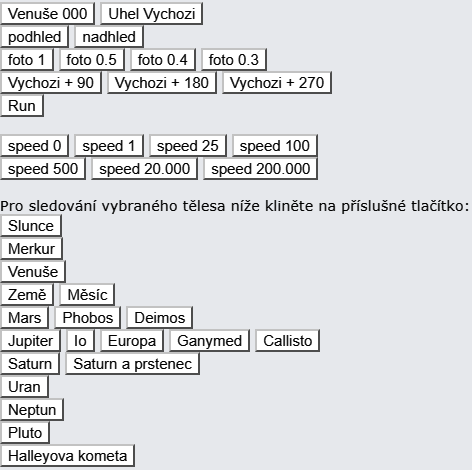
\includegraphics[width=0.8\textwidth]{img4.png}
\caption{Ukázka ovládacího rozhraní modelu}
\label{obr4}
\end{figure}

Předvedený model lze použít ve výuce~v~mateřské škole, základní škole ale~i~na gymnáziu~a~střední škole. Model lze vytvořit, ale také spustitna různých platformách,~a~pro jeho tvorbu nám postačí jakýkoli webovýprohlížeč. Univerzalita prostředí GlowScript Trinket je značná co do platforem, ale také do možností, které nám prostředí nabízí. Lze~s~ním pracovatjak kvalitativně, tak kvantitativně. Pokud se zaměříme na mezipředmětovost, pak ji samozřejmě můžeme najít mezi Fyzikou~a~ICT předmětem,nyní hovoříme~o~základní škole, gymnáziu~a~střední škole.

Další vzdělávací podtext můžeme spatřit~v~tom, že necháme žáky, abysami hledali základní parametry těles, která se nacházejí ve Sluneční soustavě.
\medskip

\nocite{*}

\printbibliography[title={Použitá literatura}] % sazba seznamu citací
\addcontentsline{toc}{chapter}{Použitá literatura} % vložení nadpisu do obsahu


\end{document}
